\section{Methods}
\label{sec:methods}
In this section, the methods used to compute the magnetic vector potential and the magnetic field
of a straight wire segment and a circular wire loop are established.

\subsection{Straight Wire Segment}
The straight wire segment is handled first.

\subsubsection{Magnetic Vector Potential}
The magnetic vector potential of a straight wire segment
only has component~$A_z$ parallel to the wire that is given by:
\begin{equation}
  A_z(\rho, z) = \frac{\mu_0 I}{4 \pi} \ln \left( \frac{1+\epsilon}{1 - \epsilon} \right)
\end{equation}
with
\begin{align}
  \epsilon =&\, \frac{L}{R_i + R_f} \\
       R_i =&\, \sqrt{\rho^2 + z^2} \\
       R_f =&\, \sqrt{\rho^2 + (1-z)^2} \, .
\end{align}
Here, we use normalized coordinates~$\rho' = \rho/L$ and~$z' = z/L$.
This leads to the following expressions for~$r_i = R_i/L$ and~$r_f = R_f/L$:
\begin{align}
  r_i =&\, \sqrt{{\rho'}^2 +      {z'}^2 } \label{eqn:r_i_default} \\
  r_f =&\, \sqrt{{\rho'}^2 + (1 - {z'})^2} \label{eqn:r_f_default} \\
  \epsilon =&\, \frac{1}{r_i + r_f} \, .
\end{align}
A common prefactor depending on the current~$I$ and~$\mu_0$ is split off:
\begin{equation}
  A_z(\rho, z) = \frac{\mu_0 I}{2 \pi} \tilde{A}_z (\rho', z')
\end{equation}
with
\begin{equation}
  \tilde{A}_z (\rho', z')
  = \frac{1}{2} \ln \left( \frac{1+\epsilon}{1 - \epsilon} \right)
  = \textrm{atanh} (\epsilon) \, .
  \label{eqn:A_z_tilde}
\end{equation}
The rest of this section can thus focus on accurate computation of $\tilde{A}_z (\rho', z')$.

The region close to the wire segment~(``near-field'') is handled by one of the following three formulations.
The parameter~$\epsilon$ approaches a value of~$1$ as the location of the evaluation point comes closer to the wire segment.
Thus, the denominator in \eqn{A_z_tilde} vanishes, leading to a logarithmic singularity in~$\tilde{A}_z$
as the evaluation point~$(\rho', z')$ gets nearer to the wire segment.
It is therefore favorable to formulate the near-field method in terms of~$(1-\epsilon)$:
\begin{align}
  1-\epsilon =&\, 1 - \frac{1}{r_i + r_f} = \frac{r_i + r_f - 1}{r_i + r_f} = \frac{r_i + r_f - 1}{(r_i + r_f - 1) + 1} = \frac{n}{n + 1}
\end{align}
with~$n \equiv r_i + r_f - 1$ approaching~$0$ as the evaluation point approaches the wire segment.
Inserting this formulation for~$1-\epsilon$ into \eqn{A_z_tilde} leads to:
\begin{align}
  \tilde{A}_{z,\mathrm{nf}} (\rho', z')
  =&\, \frac{1}{2}  \left[ \ln\left(2 - (1-\epsilon)        \right) - \ln \left(1 - \epsilon    \right) \right] \nonumber \\
  =&\, \frac{1}{2}  \left[ \ln\left(2 - \frac{n}{n + 1}     \right) - \ln \left(\frac{n}{n + 1} \right) \right] \nonumber \\
  =&\, \frac{1}{2}  \left[ \ln\left(\frac{2(n+1) - n}{n + 1}\right) - \ln \left(\frac{n}{n + 1} \right) \right] \nonumber \\
  =&\, \frac{1}{2}  \left[ \ln\left(n + 2                   \right) \cancel{- \ln\left(n + 1 \right)} - \ln \left( n \right) \cancel{+ \ln \left( n + 1 \right)} \right] \nonumber \\
  =&\, \frac{1}{2}  \left[ \ln\left(n + 2                   \right) - \ln \left( n \right) \right] \, .
\end{align}
The subscript ``nf'' was introduced to indicate that this formulation shall only be used for the near-field.
The method used to compute~$n$ still has to be switched depending to the exact location of the evaluation point:
\begin{equation}
  n = \begin{cases}
        n_{6a} &:\, z' \geq 1 \textrm{ or } \rho'/(1-z') \geq 1 \\
        n_{6b} &:\, z' \geq 0 \textrm{ and } \rho'/z' \leq 1 \\
        n_{6c} &:\, \textrm{else}
      \end{cases} \, .
\end{equation}
% A_6a start
The first special case introduces a nutritious zero~($-z' + z'$) into~$n$:
\begin{equation}
  n_{6a} = (r_i - z') + r_f + (z'-1) \, .
\end{equation}
The first contribution to~$n$ is then computed as follows:
\begin{equation}
  r_i - z' = 2 z' \sin^2(\alpha/2) / \cos(\alpha) \label{eqn:ri_zp}
\end{equation}
with $\alpha = \texttt{atan2}(\rho', z')$.
Additionally, $r_f$ is computed via \eqn{r_f_default} and $(z'-1)$ is computed directly.
% A_6a end
% A_6b start
The second special case is based on the first one and introduces another angle~$\beta$
used to compute~$r_f + (z'-1)$ directly:
\begin{equation}
  (r_f + z' - 1) = 2 (1 - z') \sin^2(\beta/2) / \cos(\beta) \label{eqn:rf_zp_1}
\end{equation}
with~$\beta = \texttt{atan2}(\rho', 1-z')$.
Then, $n$ is computed as:
\begin{equation}
  n_{6b} = (r_i - z') + (r_f + z'-1)
\end{equation}
with $(r_i - z')$ from \eqn{ri_zp} and $(r_f + z' - 1)$ from \eqn{rf_zp_1}.
% A_6b end
% A_6c start
The third special case is formulated slightly differently.
Here, $(r_f-1)$ is formulated as:
\begin{equation}
  r_f - 1 = 2 r_f \sin^2(\beta/2) - z' \label{eqn:rf_1}
\end{equation}
with $\beta$ as in the second special case
and $r_i$ and $r_f$ from \eqn{r_i_default} and \eqn{r_f_default}, respectively.
This leads to:
\begin{equation}
  n_{6c} = r_i + (r_f - 1)
\end{equation}
with $(r_f - 1)$ from \eqn{rf_1}.
% A_6c end
This concludes the methods for the near-field evaluation.
Two further special cases are considered next: $\rho' = 0$ and the combined case ($z'=0$, $z'=1$).
For the case of $\rho'=0$, the following formulation should be used:
\begin{equation}
  \tilde{A}_z (\rho'=0, z')
  = \begin{cases}
      \tilde{A}_2(z')  &:\, z' < 1 \textrm{ or } z' > 2 \\
      \tilde{A}_2b(z') &:\, \textrm{else, except } z' \in [0, 1]
    \end{cases}
\end{equation}
with
\begin{equation}
  \tilde{A}_2(z') = \textrm{atanh}\left( \frac{1}{|z'| + |1 - z'|} \right)
\end{equation}
and
\begin{equation}
  \tilde{A}_2b(z') = \frac{1}{2} \textrm{sgn}(z') \ln \left(\left| \frac{z'}{1-z'} \right| \right) \, .
\end{equation}
The following formulation should be used for the cases $z'=0$ or $z'=1$:
\begin{equation}
  \tilde{A}_z (\rho', z' \in \{0, 1\})
  = \begin{cases}
      \tilde{A}_3(\rho')  &:\, \rho' > 1 \\
      \tilde{A}_bb(\rho') &:\, \textrm{else}
    \end{cases}
\end{equation}
with
\begin{equation}
  \tilde{A}_3(z') = \textrm{atanh}\left( \frac{1}{\rho' + \sqrt{{\rho'}^2 + 1}} \right)
\end{equation}
and
\begin{align}
  \tilde{A}_3b(z') =&\, \frac{1}{2} \ln \left(\frac{\rho' c + 1 + c}{\rho' c + 2 s^2 }\right) \\
  c =&\, \cos(\alpha) = \left[{\rho'}^2 + 1 \right]^{-1/2} \\
  s =&\, \sin(\alpha/2)  \\
 \alpha =&\, \arctan(\rho') \, .
\end{align}
If none of above special cases applies,
the following general formulation is used for the ``far-field'' case:
\begin{equation}
  \tilde{A}_{z,\mathrm{ff}} (\rho', z') = \textrm{atanh}\left( \frac{1}{r_i + r_f} \right)
\end{equation}
with $r_i$ and $r_f$ from \eqn{r_i_default} and \eqn{r_f_default}, respectively.
%
% total assembly
%
The overall switching between the methods introduced above is done as follows:
\begin{equation}
  \tilde{A}_z (\rho', z')
  = \begin{cases}
      \tilde{A}_z (\rho'=0, z')             &:\, \rho' = 0 \\
      \tilde{A}_z (\rho', z' \in \{0, 1\})  &:\, z' \in \{0, 1\} \\
      \tilde{A}_{z,\mathrm{nf}} (\rho', z') &:\, z' \in ]-1, 2] \textrm{ and } \rho' < 1 \\
      \tilde{A}_{z,\mathrm{ff}} (\rho', z') &:\, \textrm{else}
    \end{cases} \, .
\end{equation}

\subsubsection{Magnetic Field}
The magnetic field of a straight wire segment
only has a tangential component~$B_\varphi$ around the wire that is given by:
\begin{equation}
  B_\varphi(\rho, z) = \frac{\mu_0 I}{2 \pi} \frac{L(R_i + R_f)}{R_f} \frac{1}{\left(R_i + R_f\right)^2 - L^2}
\end{equation}
with~$L$, $R_i$ and $R_f$ as in the previous section.
Again a normalization factor is split off:
\begin{equation}
  B_\varphi(\rho, z) = \frac{\mu_0 I}{2 \pi L} \tilde{B}_\varphi(\rho', z')
\end{equation}
with
\begin{align}
  \tilde{B}_\varphi(\rho', z')
  =&\, \frac{L^2(R_i + R_f)}{R_f} \frac{1}{\left(R_i + R_f\right)^2 - L^2} \nonumber \\
  =&\, \left(\frac{r_i}{r_f} + 1\right) \frac{1}{\left(r_i + r_f\right)^2 - 1} \, .
\end{align}









\subsection{Circular Wire Loop}
The circular wire loop is handled next.

\subsubsection{Magnetic Vector Potential}


\subsubsection{Magnetic Field}


\subsection{Transformation to Cartesian Coordinates}
Evaluation of the magnetostatic quantities~$A_\varphi$, $B_\rho$ and $B_z$ happens in cylindrical coordinates~$\rho$ and~$z$.
It is often more convenient to be able to work in Cartesian coordinates.
Figure~\ref{fig:mappingToCartesian} illustrates the setup of a circular wire loop.
\begin{figure}[htbp]
 \centering
 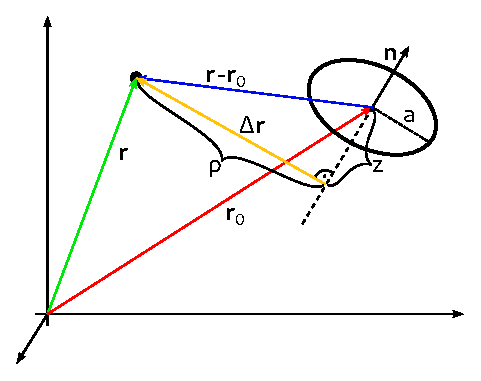
\includegraphics{img/MappingToCartesian.eps}
 \caption{Mapping the components to Cartesian coordinates for an exemplary circular wire loop.
          The loop is centered around its origin~$\mathbf{r}_0$.
          Its normal vector is denoted $\mathbf{n}$ and defines the orientation of the loop.
          The radius of the loop is denoted by~$a$.
          The evaluation location is denoted by~$\mathbf{r}$.}
 \label{fig:mappingToCartesian}
\end{figure}

The $z$-axis of the wire loop's coordinate system is defined by the normal vector~$\mathbf{n}$:
\begin{equation}
  \hat{\mathbf{e}}_z = \frac{\mathbf{n}}{|\mathbf{n}|} \, .
\end{equation}
The $z$ component of the evaluation location is thus obtained as follows:
\begin{equation}
  z = (\mathbf{r} - \mathbf{r}_0) \cdot \hat{\mathbf{e}}_z \, .
\end{equation}
The normalized $z$-coordinate $z'$ is then obtained as:
\begin{equation}
  z' = \frac{z}{a} = \frac{1}{a} (\mathbf{r} - \mathbf{r}_0) \cdot \hat{\mathbf{e}}_z \, .
\end{equation}
For the radial coordinate, first the vector~$\Delta \mathbf{r}$ is formed:
\begin{equation}
  \Delta \mathbf{r} = (\mathbf{r} - \mathbf{r}_0) - z \, \hat{\mathbf{e}}_z
\end{equation}
and the radial coordinate $\rho$ is then obtained by taking $\rho = |\Delta \mathbf{r}|$.
A unit vector in radial direction is formed as follows:
\begin{equation}
  \hat{\mathbf{e}}_\rho = \frac{\Delta \mathbf{r}}{\rho} \, .
\end{equation}
The normalized radial coordinate~$\rho'$ is then obtained as:
\begin{equation}
  \rho' = \frac{\rho}{a} = \frac{1}{a} |(\mathbf{r} - \mathbf{r}_0) - z \, \hat{\mathbf{e}}_z| \, .
\end{equation}
The magnetic field of the circular wire loop consists of two cylindrical components, namely $B_\rho$ and $B_z$.
The Cartesian magnetic field components are then computed as follows:
\begin{equation}
  \mathbf{B}(\mathbf{r}) = B_\rho \hat{\mathbf{e}}_\rho + B_z \hat{\mathbf{e}}_z \, .
\end{equation}
The magnetic vector potential only has a component in angular direction in the coordinate system of the wire loop.
The corresponding unit vector~$\hat{\mathbf{e}}_\varphi$ is then given by
$\hat{\mathbf{e}}_\varphi = \hat{\mathbf{e}}_\rho \times \hat{\mathbf{e}}_z$.
The vector potential of the circular wire loop in thus in Cartesian coordinates:
\begin{equation}
  \mathbf{A}(\mathbf{r}) = A_\varphi \hat{\mathbf{e}}_\varphi \, .
\end{equation}

\subsection{Superposition in multi-filament assemblies}
% PolygonFilament
An infinitely thin polygon filament $P$ is described by a list of $N$ points $\mathbf{x}_i$ with $i=1, ..., N$ in three-dimensional (3D) space and a current $I$.
The $(N-1)$ straight connecting lines between each two consecutive points $\mathbf{x}_i$ and $\mathbf{x}_{i+1}$ are assumed to represent the geometry of a wire which carries the current.
If the first and the last point of the polygon filament coincide, the wire forms a closed loop and $\nabla \cdot \mathbf{j} = 0$ is ensured by construction.

The magnetic vector potential $\mathbf{A}(I, \mathbf{x}_i, \mathbf{x}_{i+1}, \mathbf{x})$ and the magnetic field $\mathbf{B}(I, \mathbf{x}_i, \mathbf{x}_{i+1}, \mathbf{x})$
of the wire segments at a location $\mathbf{x}$ can be computed analytically.
The resulting contributions from each segment are superposed in order to compute the resulting magnetic field from the full length of the wire:
\begin{align}
 \mathbf{A}(\mathbf{x}) & = \sum_{i=1}^{N-1} \mathbf{A}(I, \mathbf{x}_i, \mathbf{x}_{i+1}, \mathbf{x}) \quad \mathrm{and} \\
 \mathbf{B}(\mathbf{x}) & = \sum_{i=1}^{N-1} \mathbf{B}(I, \mathbf{x}_i, \mathbf{x}_{i+1}, \mathbf{x}) \quad .
\end{align}
Computationally robust and efficient expressions for
$\mathbf{A}(I, \mathbf{x}_i, \mathbf{x}_{i+1}, \mathbf{x})$ and
$\mathbf{B}(I, \mathbf{x}_i, \mathbf{x}_{i+1}, \mathbf{x})$
are given in Ref.~\cite{hanson_hirshman_2002}.
The detailed derivation of these expressions is given below.

% multi-winding circular coil
